\documentclass[11pt,a4paper]{article}
\usepackage[margin=2.1cm]{geometry}
\usepackage{amsmath}
\usepackage{graphicx}
\usepackage{booktabs}
\usepackage{tabularx}
\usepackage{caption}
\usepackage{float}
\usepackage{parskip}
\usepackage[hidelinks]{hyperref}
\captionsetup{font=small}
\setlength{\parskip}{5pt}

\newcommand{\keybox}[1]{\par\noindent\fbox{\parbox{\dimexpr\linewidth-2\fboxsep-2\fboxrule}{\small #1}}\par}

\title{Polynomial Regression --- Assignment Report}
\author{Roll no.\ IMT2024067 \quad$\cdot$\quad Code: PyTorch\\[2pt] \small GitHub: \url{https://github.com/VishudhaSood/Assignment1_ML}}
\date{}

\begin{document}
\maketitle
\vspace{-1.5em}

\section{The task}
We get two datasets. In each one we must predict a number $y$ from some inputs, using
\textbf{only polynomial regression}. Each has 1000 training rows (with $y$) and 1000 test rows
(without $y$). The teacher scores our test predictions with \textbf{MSE} (lower is better) and
$\mathbf{R^2}$ (closer to 1 is better). The main decision is the \textbf{degree} of the polynomial.

\begin{table}[H]
\centering
\begin{tabular}{lll}
\toprule
 & var1 --- steam turbine & var2 --- thermal reservoir \\
\midrule
Inputs & 6 ($x_1 \ldots x_6$) & 3 ($x_1, x_2, x_3$) \\
Max degree allowed & 10 & 20 \\
Input values & between $-1$ and $1$ & between $-1$ and $1$ \\
$y$ in training data & from $-9.6$ to $12.4$ & from $-29.7$ to $30.2$ \\
\bottomrule
\end{tabular}
\end{table}

\textbf{What we noticed in the data.} No missing values. Many inputs are exactly $-1$ or $+1$
(the edge of the allowed range): about 30\% in var1 and 25\% in var2. The var1 \emph{test} file has
even more edge points than the training file, so we checked edge points separately (Section~5).

\section{Method}
\begin{center}
\small
\fbox{\parbox{2.3cm}{\centering 1.\ Make polynomial terms}} $\rightarrow$
\fbox{\parbox{2.3cm}{\centering 2.\ Fit with a penalty (Ridge / Lasso)}} $\rightarrow$
\fbox{\parbox{2.3cm}{\centering 3.\ Score with 5-fold CV}} $\rightarrow$
\fbox{\parbox{2.3cm}{\centering 4.\ Pick best degree + penalty}} $\rightarrow$
\fbox{\parbox{2.3cm}{\centering 5.\ Retrain on all data, predict test}}
\end{center}

\subsection{Polynomial features}
A polynomial of degree $d$ uses every term whose powers add up to at most $d$. For example with
two inputs and $d = 2$ the terms are: $1,\ x_1,\ x_2,\ x_1^2,\ x_1x_2,\ x_2^2$. The model is just a
weighted sum of these terms, so it is still \textbf{linear regression}, only on more columns. The
number of terms grows fast:

\begin{table}[H]
\centering
\begin{tabular}{lrrrrrr}
\toprule
Degree & 1 & 3 & 5 & 8 & 10 & 20 \\
\midrule
var1 (6 inputs) & 7 & 84 & 462 & 3003 & 8008 & --- \\
var2 (3 inputs) & 4 & 20 & 56 & 165 & 286 & 1771 \\
\bottomrule
\end{tabular}
\end{table}

With only 1000 rows, a high degree has more terms than rows. Plain least squares would then fit
the training data perfectly, noise included --- this is \textbf{overfitting}. A too-low degree misses
the real shape --- \textbf{underfitting}.

\keybox{\textbf{Small extra: Legendre polynomials.} Instead of raw powers $x, x^2, x^3, \ldots$ we build
the terms from Legendre polynomials $P_1(x), P_2(x), P_3(x), \ldots$ (e.g.\ $P_2 = (3x^2 - 1)/2$). They
describe \textbf{exactly the same set of polynomials}, so the model is unchanged. We use them because on
$[-1, 1]$ high powers like $x^{18}$ and $x^{20}$ look almost identical, which makes the computer's
equation solving unstable; Legendre terms do not have this problem.}

\subsection{Fitting with a penalty: Ridge and Lasso}
To stop overfitting we add a penalty on the size of the weights $w$ (regularisation):

\begin{table}[H]
\centering
\begin{tabularx}{\linewidth}{llX}
\toprule
Method & What we minimise & Effect \\
\midrule
Ridge (L2) & error $+ \lambda \sum w^2$ & shrinks all weights, keeps every term \\
Lasso (L1) & error $+ \alpha \sum |w|$ & sets useless weights to exactly 0 $\rightarrow$ keeps only some terms \\
Relaxed Lasso & Lasso first, then refit & Lasso chooses the terms; we then refit only those terms with
(almost) no penalty, so they are not shrunk too much \\
\bottomrule
\end{tabularx}
\end{table}

$\lambda$ and $\alpha$ control how strong the penalty is. Ridge has a direct formula,
\[ w = (\Phi^\top\Phi + \lambda n I)^{-1}\Phi^\top y, \]
solved with \texttt{torch.linalg.solve}. Lasso has no formula, so it is solved step by step
(gradient steps + pushing small weights to 0). The constant term (intercept) is never penalised.

\subsection{Choosing degree and penalty: 5-fold cross-validation}
We split the training rows into 5 equal parts. We train on 4 parts and measure the MSE on the
5th part, which the model has not seen, and repeat so every part is the `unseen' part once.
The average is the \textbf{CV MSE}, our estimate of the test error. We computed it for
\textbf{every degree} (1--10 for var1, 1--20 for var2), each method, and several penalty strengths,
and picked the lowest. That model was then retrained on all 1000 rows to predict the test file.

\section{var1 --- steam turbine (6 inputs)}
\begin{figure}[H]
\centering
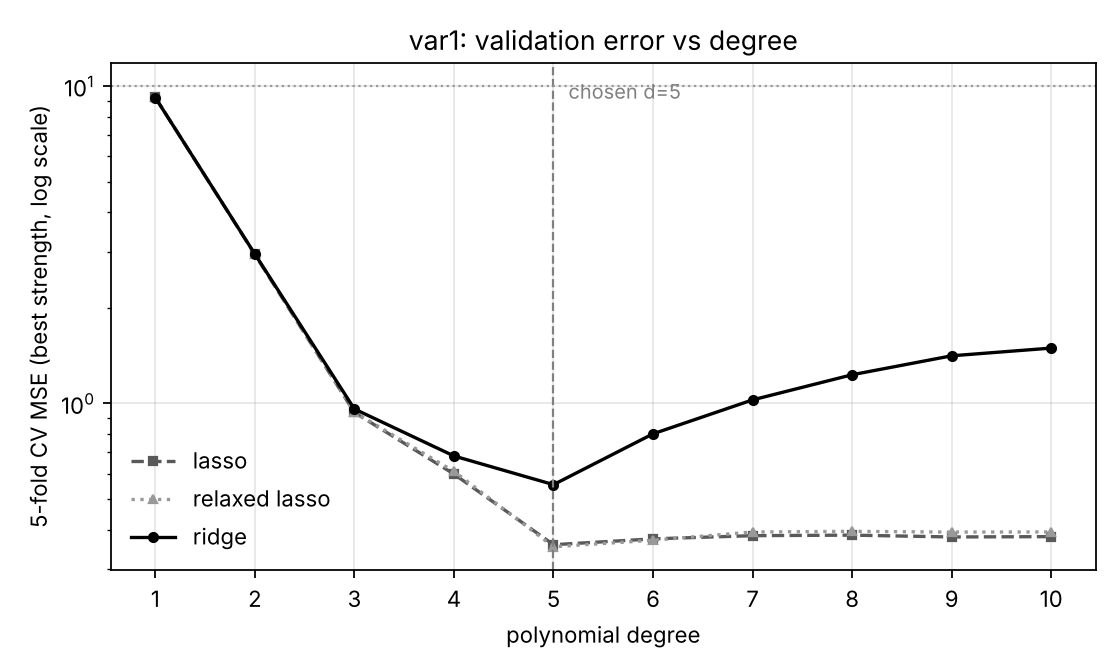
\includegraphics[width=0.7\linewidth]{plots/cv_var1.png}
\caption{CV MSE vs degree (best penalty for each method). Lower is better.}
\end{figure}

\begin{table}[H]
\centering
\begin{tabular}{rrrrr}
\toprule
Degree & No.\ of terms & Ridge & Lasso & Relaxed Lasso \\
\midrule
2 & 28 & 2.954 & 2.947 & 2.950 \\
3 & 84 & 0.959 & 0.936 & 0.938 \\
4 & 210 & 0.682 & 0.598 & 0.610 \\
5 & 462 & 0.554 & 0.358 & 0.353 \\
6 & 924 & 0.801 & 0.374 & 0.370 \\
7 & 1716 & 1.025 & 0.383 & 0.393 \\
8 & 3003 & 1.230 & 0.384 & 0.395 \\
9 & 5005 & 1.412 & 0.379 & 0.393 \\
10 & 8008 & 1.493 & 0.380 & 0.393 \\
\bottomrule
\end{tabular}
\caption{CV MSE for each degree and method.}
\end{table}

\keybox{\textbf{Chosen: degree 5, relaxed Lasso ($\alpha = 0.01$).} CV MSE $= 0.353$, CV $R^2 = 0.965$. Only 105 of the 462 possible terms are used.}

\textbf{Why degree 5?} From degree 1 to 5 the error drops a lot (lower degrees underfit). After 5 it
stops improving, so degree 5 is the simplest model that captures the pattern.

\textbf{Why Lasso and not Ridge?} At degree 5 Ridge's error is 0.55 but Lasso's is about 0.35. Ridge
keeps all 462 terms, while Lasso throws most of them away, so the real formula only uses a few
terms. Ridge also gets much worse at higher degrees (more and more useless terms), while Lasso
stays flat because it just removes them.

\section{var2 --- thermal reservoir (3 inputs)}
\begin{figure}[H]
\centering
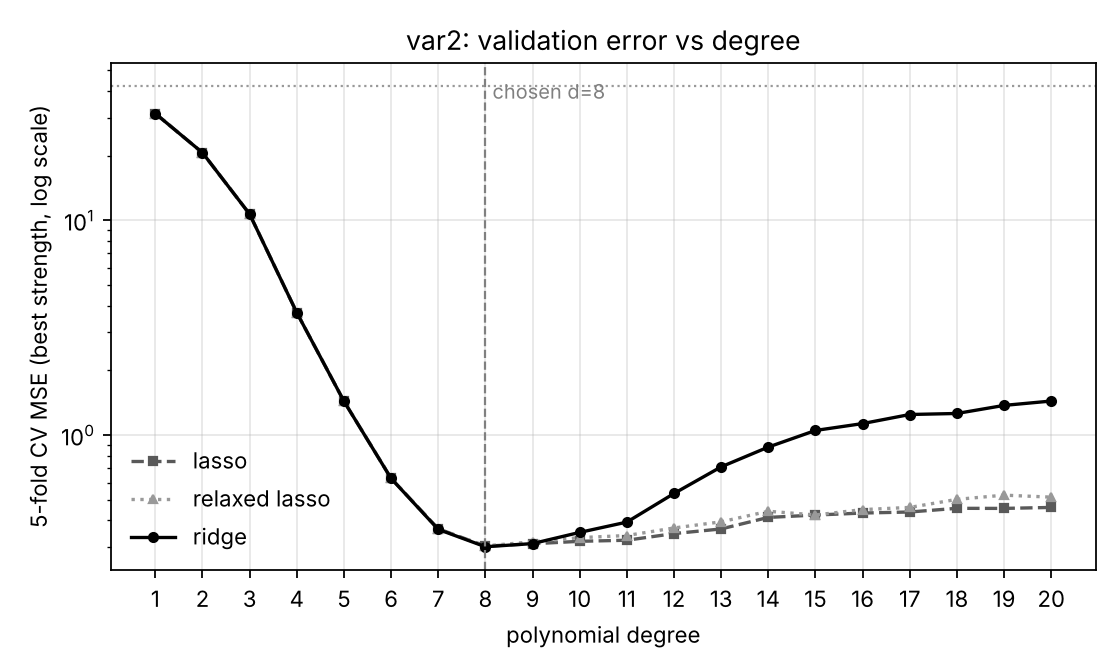
\includegraphics[width=0.7\linewidth]{plots/cv_var2.png}
\caption{CV MSE vs degree. The minimum is at degree 8.}
\end{figure}

\begin{table}[H]
\centering
\begin{tabular}{rrrrr}
\toprule
Degree & No.\ of terms & Ridge & Lasso & Relaxed Lasso \\
\midrule
4 & 35 & 3.710 & 3.710 & 3.710 \\
6 & 84 & 0.627 & 0.627 & 0.630 \\
7 & 120 & 0.363 & 0.365 & 0.363 \\
8 & 165 & 0.301 & 0.303 & 0.304 \\
9 & 220 & 0.312 & 0.311 & 0.318 \\
10 & 286 & 0.351 & 0.319 & 0.332 \\
12 & 455 & 0.533 & 0.347 & 0.368 \\
14 & 680 & 0.877 & 0.413 & 0.441 \\
16 & 969 & 1.129 & 0.432 & 0.449 \\
18 & 1330 & 1.258 & 0.455 & 0.501 \\
20 & 1771 & 1.438 & 0.459 & 0.513 \\
\bottomrule
\end{tabular}
\caption{CV MSE for selected degrees.}
\end{table}

\keybox{\textbf{Chosen: degree 8, Ridge ($\lambda = 0.001$).} CV MSE $= 0.301$, CV $R^2 = 0.993$. All 165 terms are used.}

\textbf{Why degree 8 and not 20?} Degree 20 is allowed, but the CV error is lowest at 8 and rises
after that. Above 8 the extra terms mainly fit noise (overfitting). Degree 20 Ridge is about
$5\times$ worse than degree 8.

\textbf{Why Ridge?} At degree 8 all three methods give almost the same error, so there is no sign
that terms should be removed. We keep the simplest method, Ridge, which has a direct formula.

\section{How good are the predictions?}
The real test answers are hidden, so we estimated test performance in three ways:

\begin{table}[H]
\centering
\begin{tabularx}{\linewidth}{Xll}
\toprule
Check & var1 & var2 \\
\midrule
\textbf{Hold-out test}: train on 80\% of rows, test on the other 20\% (10 random splits)
 & MSE 0.352, $R^2$ 0.964 & MSE 0.296, $R^2$ 0.993 \\
\textbf{Repeated 5-fold CV} (3 different shuffles)
 & MSE 0.353, $R^2$ 0.965 & MSE 0.303, $R^2$ 0.993 \\
\textbf{Test-like MSE}: CV error re-weighted so the share of edge points matches the test file
 & MSE $\approx$ 0.38 & MSE $\approx$ 0.31 \\
Baseline: always predict the average $y$ & MSE 9.99, $R^2$ 0 & MSE 42.1, $R^2$ 0 \\
\bottomrule
\end{tabularx}
\end{table}

All estimates agree, so the results are stable. We expect a test $R^2$ of about \textbf{0.96} for var1
and \textbf{0.99} for var2. The var1 test MSE may be slightly higher than the CV value ($\approx$0.38)
because its test file has more edge points, where errors are a bit larger
(0.40 on edge rows vs 0.33 on inner rows).

\begin{figure}[H]
\centering
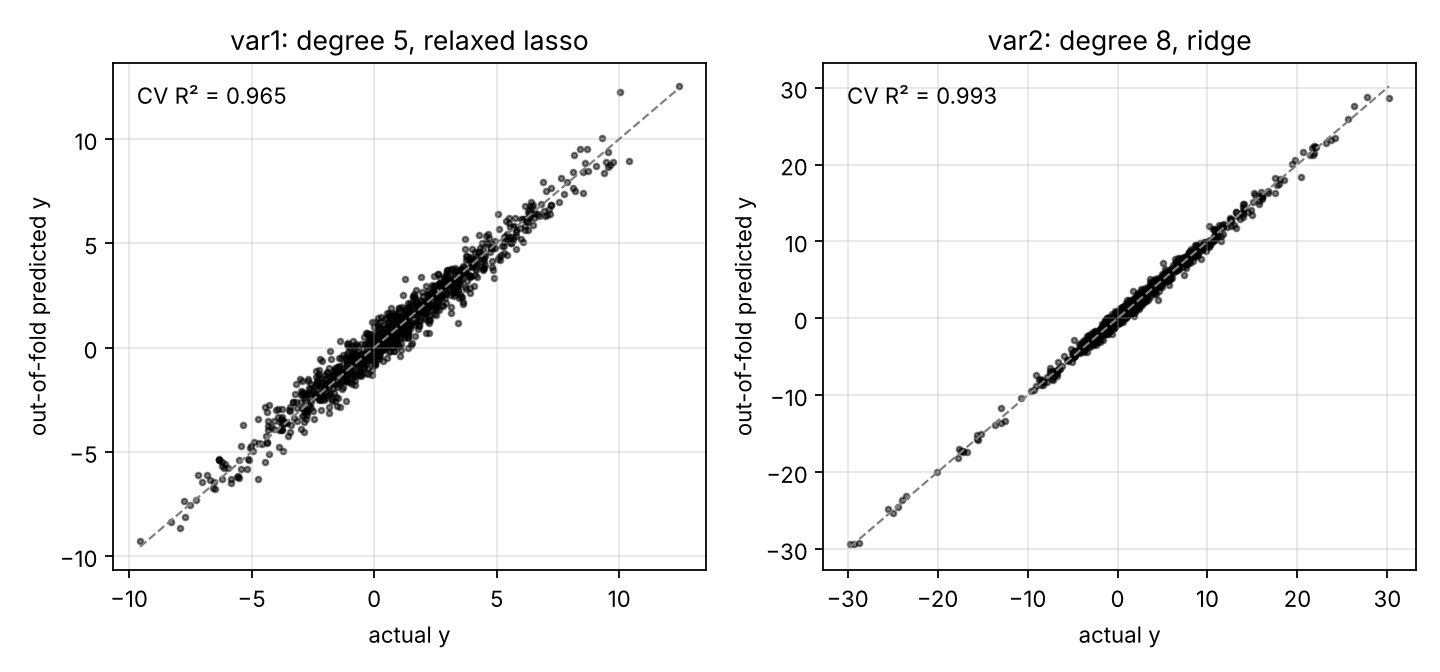
\includegraphics[width=0.78\linewidth]{plots/parity.png}
\caption{Predicted vs actual $y$ on unseen CV rows. Points lie close to the diagonal.}
\end{figure}

\begin{figure}[H]
\centering
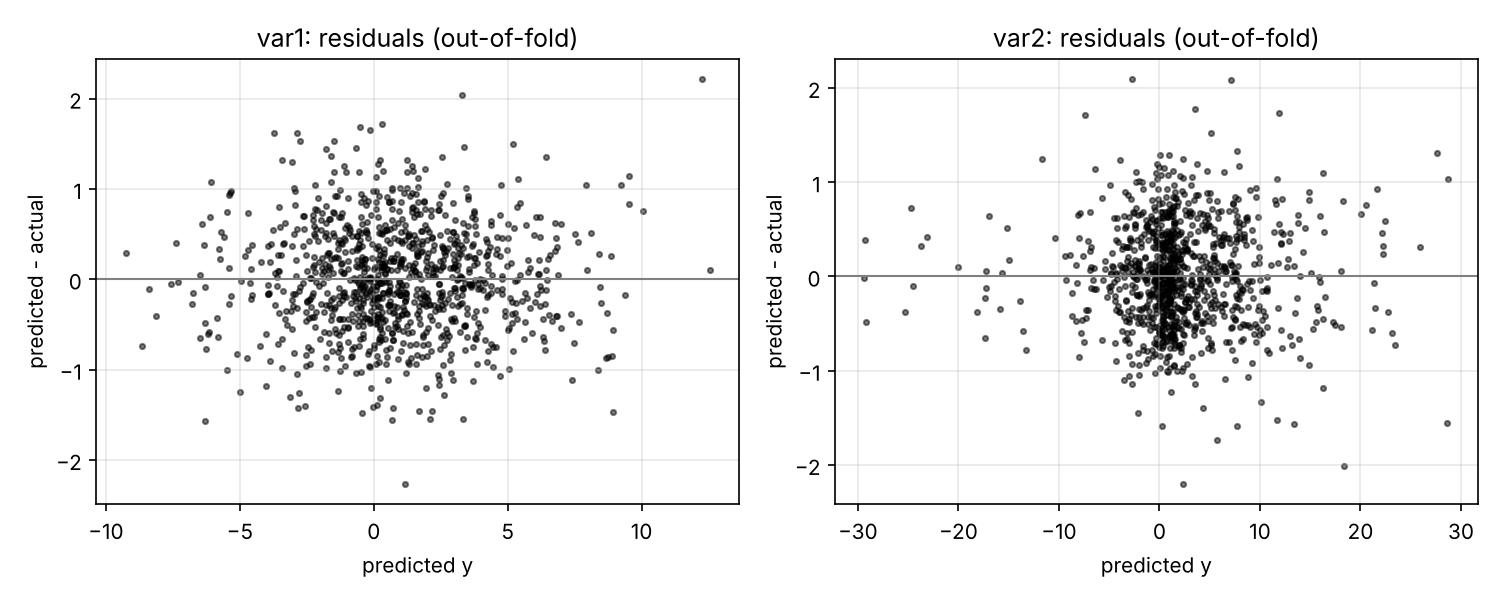
\includegraphics[width=0.78\linewidth]{plots/residuals.png}
\caption{Errors (predicted $-$ actual). They are spread randomly around 0 with no pattern, so the
model is not missing any systematic shape.}
\end{figure}

\textbf{Other checks.} Both prediction files have 1000 rows, one column $y$, no missing values and
the same row order as the test files. Re-running the code reproduces them exactly.

\section{Summary}
\begin{table}[H]
\centering
\begin{tabular}{lll}
\toprule
 & var1 & var2 \\
\midrule
Degree & 5 & 8 \\
Method & Relaxed Lasso, $\alpha = 0.01$ & Ridge, $\lambda = 0.001$ \\
Terms used & 105 of 462 & 165 of 165 \\
CV MSE / $R^2$ & 0.353 / 0.965 & 0.301 / 0.993 \\
Hold-out MSE / $R^2$ & 0.352 / 0.964 & 0.296 / 0.993 \\
Prediction file & \texttt{IMT2024067\_pred\_var1.csv} & \texttt{IMT2024067\_pred\_var2.csv} \\
\bottomrule
\end{tabular}
\end{table}

\textbf{Main takeaways.} (1) The best degree is found by cross-validation, not by taking the maximum
allowed: 5 out of 10 for var1 and 8 out of 20 for var2. (2) Regularisation is what makes
high-degree polynomials usable; Lasso helps most when only a few terms matter (var1).
(3) Hold-out and CV estimates agree, so we expect similar errors on the hidden test set.

\textbf{Code} (GitHub: \url{https://github.com/VishudhaSood/Assignment1_ML}): \texttt{polyreg.py} model, \texttt{train.py} degree search + predictions,
\texttt{validate.py} checks, \texttt{make\_plots.py}, \texttt{make\_report.py}.

\end{document}
